\section{Implementation}
\label{sec:implementation}

The following sections detail the implementation of the \ac{grs} and \ac{acc} components, resulting in a complete \ac{poc} of the \ac{gr}-based access control system. 

Several reference are made to things including buffer sizes, counters, and threshold values throughout. The following list provides a summary of what these variables were set to in this implementation, for reference.

\begin{itemize}
	\item References to 'Buffer Size', 'Max Frame Count' or similar indicate a value of 30
	\item References to 'Minimum Contour Area' indicate a value of 500
	\item References to 'Confidence Threshold' or similar indicate a value of 75\%
	\item References to 'Normalised Width' and 'Normalised Height' indicate a value of 88 and 128 respectively
\end{itemize}


\subsection{Image Processing and Gait Energy Image (GEI) Creation}
\label{subsec:image-processing-gei}

The \ac{gei} creation process, designed in Section \ref{subsec:gei-creation}, was the first to be implemented.
This is a component of the \ac{acc} (designed in Section \ref{subsec:access-control-client-design} and implemented in Section \ref{subsec:access-control-client-implementation}) but was developed first due to being the core component of this project; producing the abstracted gait cycle representations that enable person identification.

Following the design steps outlined in Section \ref{subsec:gei-creation}, this process was implemented to enable \ac{gei} generation from video footage.
The following subsections describe how each stage of the process was implemented.

\subsubsection{Capturing Camera Input}

To capture input from the camera using Python, the \ac{cv2} library is utilized. It provides functionality allowing frames to be read using the \codeword{VideoCapture} class and its \codeword{read} method.
A basic example of this functionality is shown in Listing \ref{lst:video-capture-code} below:

\begin{code}
capture = cv2.VideoCapture(camera_id=0)

def get_frame():
	ret, frame = capture.read()
	if ret:
		return frame
	return None

while True:
	frame = get_frame()
\end{code}
\captionof{listing}{OpenCV (CV2) 'VideoCapture' Class Usage}
\label{lst:video-capture-code} \vspace{10pt}

To improve robustness, adhere to \ac{oop} principles, and maintain separation of concerns, this functionality is encapsulated in a \codeword{Camera} class.
This allows frame capture to run in a separate thread, initiated using the class' \codeword{start} method, with the most recent frame retrieved using its \codeword{get\_frame} method. \textit{The final implementation of the \codeword{Camera} class can be seen in Appendix \ref{app:camera-implementation}.}


\subsubsection{Background Subtraction and Person Detection}
\label{subsec:background-subtraction-and-person-detection}

The person detection and background subtraction stages defined in Section \ref{subsec:gei-creation} have been combined, with efficient person detection actually becoming easier after irrelevant information (the background) is removed.

Before background subtraction is performed, a simple 'background model' is created describing what the average background looks like.
This is done by buffering a number $N$ frames (collected using the \codeword{Camera} class' \codeword{get\_frame} method), converting them to grayscale, and using the 'NumPy' library's \codeword{median} function to compute the background model by averaging the pixel intensity of buffered frames.
For example, let $I_k(x,y)$ be the intensity of the $k^th$ frame at pixel $(x,y)$ for $k=1,2,...,N$. The background model $B(x,y)$ is computed as: \[ B(x,y) = median(I_1(x,y),I_2(x,y),...,I_N(x,y))\] Where:

\begin{itemize}
	\item $N$ is the background frame buffer size
	\item $B(x,y)$ is the average intensity (0-255) at pixel $(x,y)$
\end{itemize}

After computing the background model, the frame buffer is cleared, and the model is stored as a variable \codeword{background\_model}.
Background subtraction is then performed on subsequent frames, with the first steps involving converting the input frame to grayscale and applying a light Gaussian blur. This simplifies processing and reduces computational load by reducing noise. Following this, more \ac{cv2} functions are used to:

\begin{enumerate}
	\item Calculate the 'absolute difference' between the background model and input frame: \codeword{diff = cv2.absdiff(background\_model, gray)}
	\item Apply a 'binary threshold' of 25 to the difference to isolate the likely foreground: \codeword{\_, binary = cv2.threshold(diff, 25, 255, cv2.THRESH\_BINARY)}
	\item Perform 'morphological closing' to fill small gaps in the foreground (noise reduction): \codeword{silhouette = cv2.morphologyEx(binary, cv2.MORPH\_CLOSE, np.ones((5, 5), np.uint8))}
	\item Identify all of the contours (shapes) present in the foreground: \codeword{contours, \_ = cv2.findContours(silhouette, cv2.RETR\_EXTERNAL, cv2.CHAIN\_APPROX\_SIMPLE)}
\end{enumerate}

After separating foreground from background and identifying contours, any contours below a specified size \codeword{MIN\_CONTOUR\_AREA} are removed from the list to further reduce noise.
A new frame is then created containing the remaining contours.

Finally, the largest contour in the list (most likely to be a person) is identified, and its dimensions are evaluated to determine whether it has an acceptable \ac{ar}, where $AR=\frac{width}{height}$.
In this implementation, a valid \ac{ar} is defined as being between 1.5 and 3.5, with a bounding box defined if so, indicating the region of interest that the person is assumed to be in. 
If the largest contour does not have an acceptable \ac{ar}, the process does not return a bounding box, indicating that no person is detected in the frame.

This process allows for simple and efficient background subtraction and person detection \textit{per frame}.
While it is not guaranteed that the largest contour with an acceptable \ac{ar} is a person, the assumption can and has been made in this controlled environment.
Figure \ref{fig:bg-subtraction-results} below illustrates the output achieved using the information provided by this process.

\begin{figure}[H]
	\centering
	\begin{minipage}{0.48\textwidth}
		\centering
		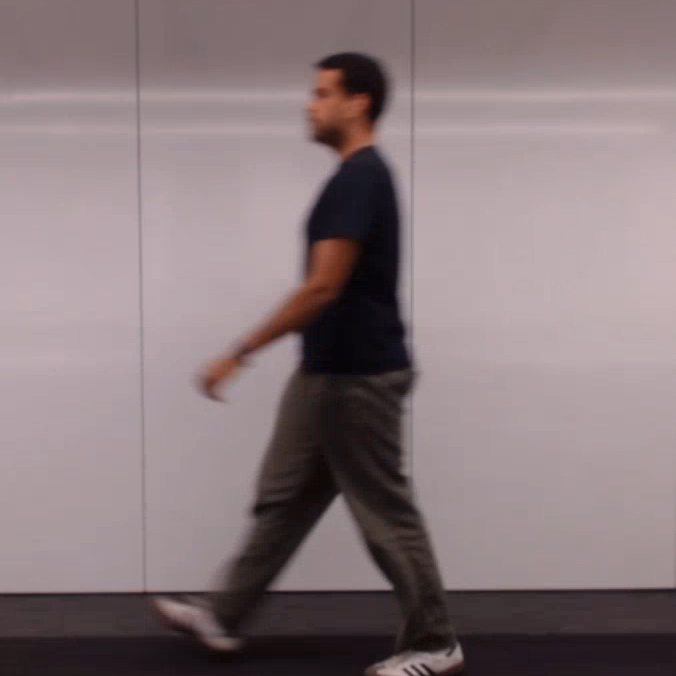
\includegraphics[width=\linewidth]{assets/bg-sub_1.png}
		\subcaption{Input Frame}
	\end{minipage}
	\hfill
	\begin{minipage}{0.48\textwidth}
		\centering
		
\includegraphics[width=\linewidth]{assets/bg-sub_2.png}
		\subcaption{Silhouette Contours}
	\end{minipage}
	\caption{Background Subtraction Process Results}
	\label{fig:bg-subtraction-results}
\end{figure}

In the final \ac{acc} implementation, this process is encapsulated within the private \codeword{\_extract\_silhouette} method of the \codeword{GaitProcessor} class --- see Appendix \ref{app:gait-processor-implementation}.

\subsubsection{Silhouette Normalisation}
\label{subsec:silhouette-normalisation}

Following silhouette extraction, normalisation is applied to crop and resize silhouettes to a standard resolution and horizontally align them based on the subject's centre of mass (i.e., the head and torso, which are most consistently positioned). \textit{Note:} this and subsequent stages are only executed if a region of interest is defined by the silhouette extraction stage.

The first step in normalisation is to crop the silhouette.
This is done using the bounding box values calculated previously to 'slice' the NumPy array representation of the silhouette based on the bounding box's \codeword{width}, \codeword{height}, \codeword{y}, and \codeword{x} position (top left corner): \codeword{person\_region = silhouette[y:y+h,x:x+w]}.

Once the figure has been isolated from the greater silhouette frame, the bounding box is tightened by identifying non-zero pixels and redefining the boundary to the smallest possible size that still encloses the silhouette, removing unnecessary space.

The silhouette's centre of mass \codeword{cx} is then calculated by averaging the x-coordinates of all non-zero pixels, providing an estimate of the subject's geometric centre along the x-axis:
\[ cx=\left\lfloor{\frac{1}{N}}\sum_{i=1}^{N}x_i\right\rfloor \] Where:

\begin{itemize}
	\item $N$ is the total number of non-zero pixels in the region
	\item $x_i$ is the x-coordinate of the $i^th$ non-zero pixel
\end{itemize}

Based on the estimated centre of mass, the silhouette is inserted into a new frame (of equal height) and horizontally aligned. This ensures consistent alignment across all silhouettes before they are used to produce the \ac{gei}, allowing for more consistent feature extraction and identity classification.

Finally, the NumPy array representing the silhouette is sliced to resize and crop it to a standard resolution --- defined by the \codeword{NORMALISED\_HEIGHT} and \codeword{NORMALISED\_WIDTH} constants.
Figure \ref{fig:normalisation-result} below shows (a) the initial silhouette, and (b) the normalised output. This step is repeated for every frame captured, with each normalised silhouette appended to a buffer maintained using a fixed size list \codeword{aligned\_buffer}, and subsequently used to create the \ac{gei}.

\begin{figure}[H]
	\centering
	
\includegraphics[width=0.25\textwidth]{assets/norm_result.png}
	\caption{Normalisation Process Results}
	\label{fig:normalisation-result}
\end{figure}

In the final \ac{acc} implementation, this process is encapsulated within the private \codeword{\_align\_silhouette} method of the \codeword{GaitProcessor} class --- see Appendix \ref{app:gait-processor-implementation}.

\subsubsection{Silhouette Averaging}
\label{subsec:silhouette-averaging}

The final step in \ac{gei} creation is to average the set of normalised silhouettes created by the steps defined above.
Every time a normalised silhouette is produced, it is appended to the sliding \codeword{aligned\_buffer}.
Once at the required size, the silhouettes are stacked and averaged to form the \ac{gei}, representing spatial and temporal information about the subject's gait pattern.

If no prior \ac{gei} exists in memory (i.e., on the first run), the \ac{gei} is computed as the mean of all silhouettes in the buffer:
\[ GEI = \frac{1}{N}\sum_{k=1}^{N}I_k \] Where:

\begin{itemize}
	\item $GEI$ is the stack of averaged silhouettes - the \acf{gei}
	\item $I_k$ is the aligned silhouette at frame $k$
	\item $N$ is the number of silhouettes in the buffer
\end{itemize}

However, if there is an existing \ac{gei}, a 'weighted update' is performed using a configurable \ac{ema}. 
This helps the \ac{gei} adapt at a defined rate over time as new silhouettes are captured and the buffer is updated:
\[ GEI_{new} = (1-\alpha)\cdot GEI_{prev}+\alpha\cdot\bar{S} \] Where:

\begin{itemize}
	\item $\bar{S}$ is the mean silhouette from the buffer
	\item $\alpha\in[0,1]$ is the weighted update rate (lower = slower)
	\item $GEI_{prev}$ is the previous \ac{gei}
	\item $GEI_{new}$ is the new \ac{gei} 
\end{itemize}

In this implementation, a low (0.2) $\alpha$ value is used which prioritises older silhouettes over new ones, minimising the potential impact of intermittent noisy or inconsistent frames. The closer the $\alpha$ value is to 1.0, the faster the \ac{gei} is adapted to new silhouette input.

The output of this step is a \ac{gei} image representing the subject's gait cycle over $k$ frames.
These are used by the \ac{grs} to perform feature extraction and identity classification.
Figure \ref{fig:gei-result} below shows an example of a \ac{gei} created by applying this process to a sequence of normalised silhouettes from the GRIDDS dataset \parencite{nunesGRIDDSGaitRecognition2019}.

\begin{figure}[H]
	\centering
	\reflectbox{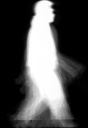
\includegraphics[width=0.25\textwidth]{assets/raff-gei.jpg}}
	\caption{Example Silhouette Averaging Result}
	\label{fig:gei-result}
\end{figure}

In the final \ac{acc} implementation, this process is encapsulated within the private \codeword{\_update\_gei} method of the \codeword{GaitProcessor} class --- see Appendix \ref{app:gait-processor-implementation}.
All methods used in the \ac{gei} creation process are called from within the \codeword{GaitProcessor}'s public \codeword{process\_frame} method.
This method is invoked by the \ac{acc}'s main thread (see Section \ref{subsec:access-control-client-implementation}) when a new camera frame is retrieved, returning both the non-normalised silhouette frame and the current \ac{gei}.

\subsection{Access Control Client}
\label{subsec:access-control-client-implementation}

The \ac{acc} leverages the camera frame capture and \ac{gei} creation process to provide the user with a view of what is occurring, following the designs outlined in Section \ref{subsubsec:client-ui-design}, where a preview of the live feed, isolated silhouette, and \ac{gei} are displayed.
It also communicates with the \ac{grs} to support registration of \ac{gei}-based identities and receive classification results of created or input \acp{gei}, using the results and associated access rule for access provision (rule = True AND confidence > 75\%).

The (Python) Flask web framework is used to serve the front-end \ac{ui}, and handle routing and user requests on the back-end. \acp{ws} (Socket.IO) are used to enable efficient data transmission between the front and back-end, continuously updating the three video views and classification results with less network overhead than traditional HTTP requests.

\subsubsection{Application State Tracking}
\label{subsubsec:application-state-tracking}

To streamline updates across the client, such as resetting the average background model for background subtraction from the front-end, tracking the number of frames processed, or the current \ac{gei}, a \codeword{state} module has been implemented which simply enables shared use of values across back-end functions. 

\begin{code}[minted language=python]
state = {
	"background_init": False, # True when background model has been created
	"reset_requested": False, # True when reset button is pressed
	"frame_counter": 0, # max 30 in this implementation
	"gei_buffer": None, # numpy array representing the current GEI
	"last_saved_gei": None, # last GEI sent for classification
}
\end{code}
\captionof{listing}{Default Access Control Client State Configuration}
\label{lst:state-configuration} \vspace{10pt}

The values in the state tracking dictionary shown in Listing \ref{lst:state-configuration} above are utilized throughout the client as follows:

\begin{itemize}
	\item \codeword{background\_init}: Set to \codeword{True} by the main thread when the \codeword{GaitProcessor} class has finished creating the averaged background model (see)
	\item \codeword{reset\_requested}: Set to \codeword{True} by the web server thread when a request is received from the front-end due to a user pressing the 'Reset Background' button
	\item \codeword{frame\_counter}: Incremented by the main thread every time a new frame is processed, reset to zero by the identification thread (see Section \ref{subsubsec:identity-classification-thread}) every time a \ac{gei} is sent for classification.
	\item \codeword{gei\_buffer}: Set by the main thread every time a frame is processed and \ac{gei} returned by the \codeword{GaitProcessor}, accessed by the identification thread when retrieving the current \ac{gei} for classification
	\item \codeword{last\_classified\_gei}: Stores the last \ac{gei} sent for classification, used by the identification thread to determine whether the current \ac{gei} has already been classified
\end{itemize}

\subsubsection{Client for Gait Recognition Server API}
\label{subsec:server-api-client-implementation}

The \ac{grs} designed in Section \ref{subsec:gait-recognition-server-design} and implemented in Section \ref{subsec:gait-recognition-server-implementation} provides two \ac{api} endpoints allowing the client to either:
(1) Register \ac{gei}-based identities or (2) Submit a \ac{gei} for classification.
To abstract the use of this in the \ac{acc}, a class \codeword{ServerAPIClient} was created, providing two methods: \codeword{classify\_gei} and \codeword{register\_gei} which are used to submit requests to the respective endpoints.

The \codeword{register\_gei} method, shown in Listing \ref{lst:register-gei-method}, accepts a \ac{gei} and identity label string before encoding the \ac{gei} as Base64 and \codeword{POST}ing a \ac{json} payload containing the \ac{gei} and label:
\codeword{{gei: ..., label: ...}} to the \ac{grs}' \codeword{/api/register} endpoint. 

\begin{code}
def register_gei(self, gei_image: bytes, label: str):
	try:
		gei_base64 = base64.b64encode(gei_image).decode("utf-8")
		payload = {"label": label, "gei": gei_base64}
		response = requests.post(self.register_endpoint, json=payload)

		if response.status_code == 200:
			return True, None
		else:
			...
	except: 
		...
\end{code}
\captionof{listing}{Server API Client register\_gei Method Logic}
\label{lst:register-gei-method} \vspace{10pt}

The \codeword{classify\_gei} method, shown in Listing \ref{lst:classify-gei-method}, accepts a Base64-encoded \ac{gei} as input, before \codeword{POST}ing a \ac{json} payload containing the \ac{gei}:
\codeword{\{gei: ...\}} to the \ac{grs}' \codeword{/api/classify} endpoint. The \ac{grs} responds with a \ac{json} object containing the predicted label (person), confidence (percentage), and access rule, which the method returns.

\begin{code}
def classify_gei(self, gei_base64: str):
	try:
		response = requests.post(self.classify_endpoint, json={"gei": gei_base64})
		
		if response.status_code == 200:
			return response.json(), None
		else:
			...
	except:
		...
\end{code}
\captionof{listing}{Server API Client classify\_gei Method Logic}
\label{lst:classify-gei-method} \vspace{10pt}

Implementation of this class enabled the separation of concerns and ensured adherence to the \ac{dry} coding principles,
as these methods are used in several places throughout the client codebase.

\subsubsection{Frame Capture, Processing, and Transmission}
\label{subsubsec:frame-capture-processing-and-transmission}

The \textit{main} thread of the \ac{acc} loops continuously and leverages the \codeword{Camera} and \codeword{GaitProcessor} classes defined in Section \ref{subsec:gei-creation} to capture frames,
isolate silhouettes, and create \acp{gei}, updating the front-end view with every new frame.

When the \ac{acc}'s \codeword{main} function is called, a new instance of the \codeword{Camera} class is created,
and video capture is started by calling the class' \codeword{start} method.
Following this, a new instance of the \codeword{GaitProcessor} class is created with the \codeword{buffer\_size} set to thirty (30) frames, as illustrated in Listing \ref{lst:camera-class-usage} below:

\begin{code}
cam = Camera(camera_id=0)
cam.start()
processor = GaitProcessor(buffer_size=30)
\end{code}
\captionof{listing}{Example 'Camera' and 'GaitProcessor' Class usage}
\label{lst:camera-class-usage} \vspace{10pt}

The main loop begins by retrieving the most recent video frame (\codeword{frame0}) and calling the \codeword{GaitProcessor}'s \codeword{process\_frame} method which returns the non-normalised silhouette (\codeword{frame1}), and the current \ac{gei} (\codeword{frame2}).
All three frames are then encoded as JPEG \codeword{cv2.imencode(".jpg", current\_gei)}, then as Base64 \codeword{base64.b64encode(buffer).decode("utf-8")} before being transmitted to the front-end over the \ac{ws} using the endpoint defined by their frame name: $frame[0,1,2]$ --- see Listing \ref{lst:frame-transmission} below:

\begin{code}
for i, img in enumerate([frame, silhouette, gei]): # frame0, frame1, frame2
	_, buffer = cv2.imencode(".jpg", img) # encode as jpeg
	img_encoded = base64.b64encode(buffer).decode("utf-8") # encode as base64
	socketio.emit(f"frame{i}", img_encoded) # transmit to front-end
\end{code}
\captionof{listing}{'Live', 'Silhouette', and 'GEI' Frame Transmission via \ac{ws}}
\label{lst:frame-transmission} \vspace{10pt}

On the front-end, \ac{js} is used to listen for data received on either of the three frame endpoints (see Listing \ref{lst:frame-recieve}), updating the associated front-end HTML \codeword{img} tag's \codeword{src} attribute with the Base64 encoded frame in the format \codeword{data:image/jpeg;base64,<base64\_frame>}.

\begin{code}[minted language=javascript]
socket.on('frame0', data => {
	frame0.src = 'data:image/jpeg;base64,' + data;
});
...+2 for frame1 and frame2
\end{code}
\captionof{listing}{JavaScript WebSocket Listener for Receiving Frames}
\label{lst:frame-recieve} \vspace{10pt}

The final action in the main loop is to sleep for 0.03 seconds.
This targets a frame-rate of around 30 frames per second; $0.03 \cdot 30 \approx 1$.
A check also exists to ensure a user is present on the main page before camera frames are processed, saving unnecessary use of resources.

This fulfills the \ac{acc} ACF1 and ACF2 requirements, abstracting movement data, captured using \ac{cv} techniques into \acp{gei} before they are transmitted.

\subsubsection{Identity Classification Thread}
\label{subsubsec:identity-classification-thread}

The identity classification process defined in Section \ref{subsubsec:person-identification} has been implemented as a separate thread within the \ac{acc}. This is because it requires no user interaction and is intended to operate passively.

The classification loop starts by checking the 'state' of the \ac{acc}, evaluating the state's \codeword{frame\_counter} value to determine whether it is greater than or equal to the defined interval of thirty (30) frames.
If that is the case, the current \ac{gei} and last checked \ac{gei} are retrieved from state storage, and a check is performed to determine whether or not they differ using the \codeword{is\_different} function which performs a simple not-equal-to comparison.

If the \ac{gei} has been updated since classification was last performed, the state is updated with the new \ac{gei} set to the last checked \ac{gei}, the frame is encoded as a JPEG image and then into Base64, before a \codeword{classify\_gei} request: \codeword{response, message = api\_client.classify\_gei(gei\_base64)} is made to the \ac{grs} using the \codeword{ServerAPIClient} class (defined in Section \ref{subsec:server-api-client-implementation}).
If a valid response is received, the details are transmitted to the front-end over the \codeword{status} \ac{ws} endpoint: \codeword{socketio.emit("status", response)}.
The front-end evaluates the response, and if the prediction confidence is at or above the threshold of 75\%, the classification result is displayed to the user (see Section \ref{subsubsec:acc-user-interface}) using the \ac{js} shown below in Listing \ref{lst:status-listener}. 

\begin{code}[minted language=javascript]
socket.on('status', (data) => {
	if (data.confidence < 75) {
		confidence.textContent = 'N/A';
		access.textContent = 'Denied';
		access.classList.toggle('access-denied', true);
		person.textContent = 'Unknown';
		return;
	}

	person.textContent = data.person;
	access.textContent = data.access ? 'Granted' : 'Denied';
	access.classList.toggle('access-denied', !data.access);
	confidence.textContent = `${data.confidence}%`;
});
\end{code}
\captionof{listing}{Front-End JavaScript Listener for Receiving Classification Updates}
\label{lst:status-listener} \vspace{10pt}

Finally, the \codeword{frame\_counter} state value is reset to zero (0) before the loop restarts.
The identity classification thread in its entirety can be seen in Appendix \ref{app:identity-classification-thread-implementation}.
This fulfills the \ac{acc} ACF3 requirement, providing passive and continuous identity classification.

\subsubsection{Identity Registration Process}
\label{subsubsec:identity-registration-process}

The identity registration process is triggered from the front-end but is handled by a \ac{ws} endpoint on the back-end.
When the user presses the 'Save Identity' button, a \ac{js} function is triggered which prompts the user to enter a label for the identity, before transmitting the label and \ac{gei} over the \ac{ws} to the back-end,
shown in Listing \ref{lst:save-identity-function} below.

\begin{code}[minted language=javascript]
saveBtn.addEventListener('click', () => {
	const label = prompt('Enter label for this GEI:');
	if (label) {
		socket.emit('save', { label: label, gei: window.latestGEI });
	}
});
\end{code}
\caption{JavaScript Button-Click Handler for Saving \ac{gei}-based Identity}
\label{lst:save-identity-function}

The request to the back-end is handled by the client's \codeword{handle\_save\_gei} Socket.IO \ac{ws} endpoint, which sends a \codeword{register\_gei} request \codeword{api\_client.register\_gei(gei\_bytes, label)} to the \ac{grs} using the \codeword{ServerAPIClient} class.
The \ac{grs}-side logic for this process is discussed in Section \ref{subsec:gait-recognition-server-implementation}.

This fulfills the \ac{acc} ACF7 requirement, allowing the user to submit a captured \ac{gei} for registration with.

To support control of identity registration, a 'Reset Background' button also exists on the front-end.
When pressed, it triggers a \codeword{reset} request to the back-end via the \codeword{handle\_reset\_background} Socket.IO \ac{ws} endpoint, which modifies the state's \codeword{reset\_requested} value to \codeword{True}.
A check is performed once per loop in the main thread which invokes the \codeword{GaitProcessor}'s \codeword{reset\_background} method (see Appendix \ref{app:gait-processor-implementation}) if \codeword{reset\_requested} is \codeword{True}. 
This clears and reinitialised the background model based on the camera's current view.

\subsubsection{Manual Identity Classification}
\label{subsubsec:manual-classification-implementation}

The manual identity classification feature enables isolated demonstration of this system's \ac{gei} matching functionality.
The user is able to upload an image on the front-end's 'Manual Classification' page which is sent to the back-end before the \codeword{ServerAPIClient}'s \codeword{classify\_gei} method is used to request classification results from the \ac{grs} in the same way as live classification.

On the front-end, image submission is handled by a \ac{js} function, \codeword{handleImageInput}. This function reads the uploaded image file, converts it to Base64, and sends it to the back-end's \codeword{/api/classify} endpoint via a \codeword{POST} request. 
Upon receiving the response, it updates the classification result fields and the displayed image preview. The key functionality for this is shown in Listing \ref{lst:manual-classification-function} below: 

\begin{code}[minted language=javascript]
const response = await fetch('/api/classify', {
	method: 'POST',
	body: JSON.stringify({
		gei: base64Image
	})
});
const result = await response.json();

person.textContent = result.person;
confidence.textContent = `${result.confidence}%`;
access.textContent = result.access ? 'Granted' : 'Denied';
access.classList.toggle('access-denied', !result.access);

previewImage.src = reader.result;
\end{code}
\captionof{listing}{JavaScript Function for Manual \ac{gei} Classification}
\label{lst:manual-classification-function} \vspace{10pt}

\textit{Note:} This purposefully does not implement the prediction confidence threshold check as it is intended to be used for demonstration purposes in isolation, where it may be more valuable to display the result regardless.

The \ac{acc}'s back-end implementation of the \codeword{/api/classify} endpoint shown in Listing \ref{lst:classify-endpoint-implementation} below, accepts the Base64-encoded image, passes it to the server-side \codeword{/api/classify} endpoint, and returns the results as \ac{json}.

\begin{code}
@routes.route("/api/classify", methods=["POST"])
def classify_gei():
	try:
		data = request.get_json()
		response, _ = api_client.classify_gei(data["gei"])
		return jsonify(response), 200
	except Exception as e:
		...error handling
\end{code}
\captionof{listing}{Server '/api/classify' Endpoint Implementation}
\label{lst:classify-endpoint-implementation} \vspace{10pt}

This feature supports testing and demonstration of the system's classification pipeline without relying on live camera input, meeting the \ac{acc} ACF9 requirement.
It also aids in debugging and validation by allowing the user to test individual \ac{gei} samples manually and enables the efficacy evaluation detailed in Chapter \ref{chap:results-and-evaluation}.


\subsubsection{User-Interface}
\label{subsubsec:acc-user-interface}

The \ac{acc}'s front-end --- the two pages designed in Section \ref{subsubsec:client-ui-design} --- is built using HTML (with the Jinja2 templating engine) and CSS, with \ac{js} used to modify page content and interface with the back-end where necessary; resetting the \codeword{GaitProcessor} background model, saving a \ac{gei}-based identity, or manually submitting a \ac{gei} for classification.

The 'Live Classification' (index) page, shown in the screenshot in Figure \ref{fig:live-ui}, features three views displaying the stages of \ac{gei} creation, which are updated using \ac{js}.
It also features text areas that display classification results when received from the \ac{grs}, also updated using \ac{js}.
Additionally, the page includes buttons for resetting the \codeword{GaitProcessor} background model on the back-end and saving a \ac{gei} sample, both of which are handled by \ac{js} event listeners, detailed in Section \ref{subsec:access-control-client-implementation}.

\begin{figure}[H]
	\centering
	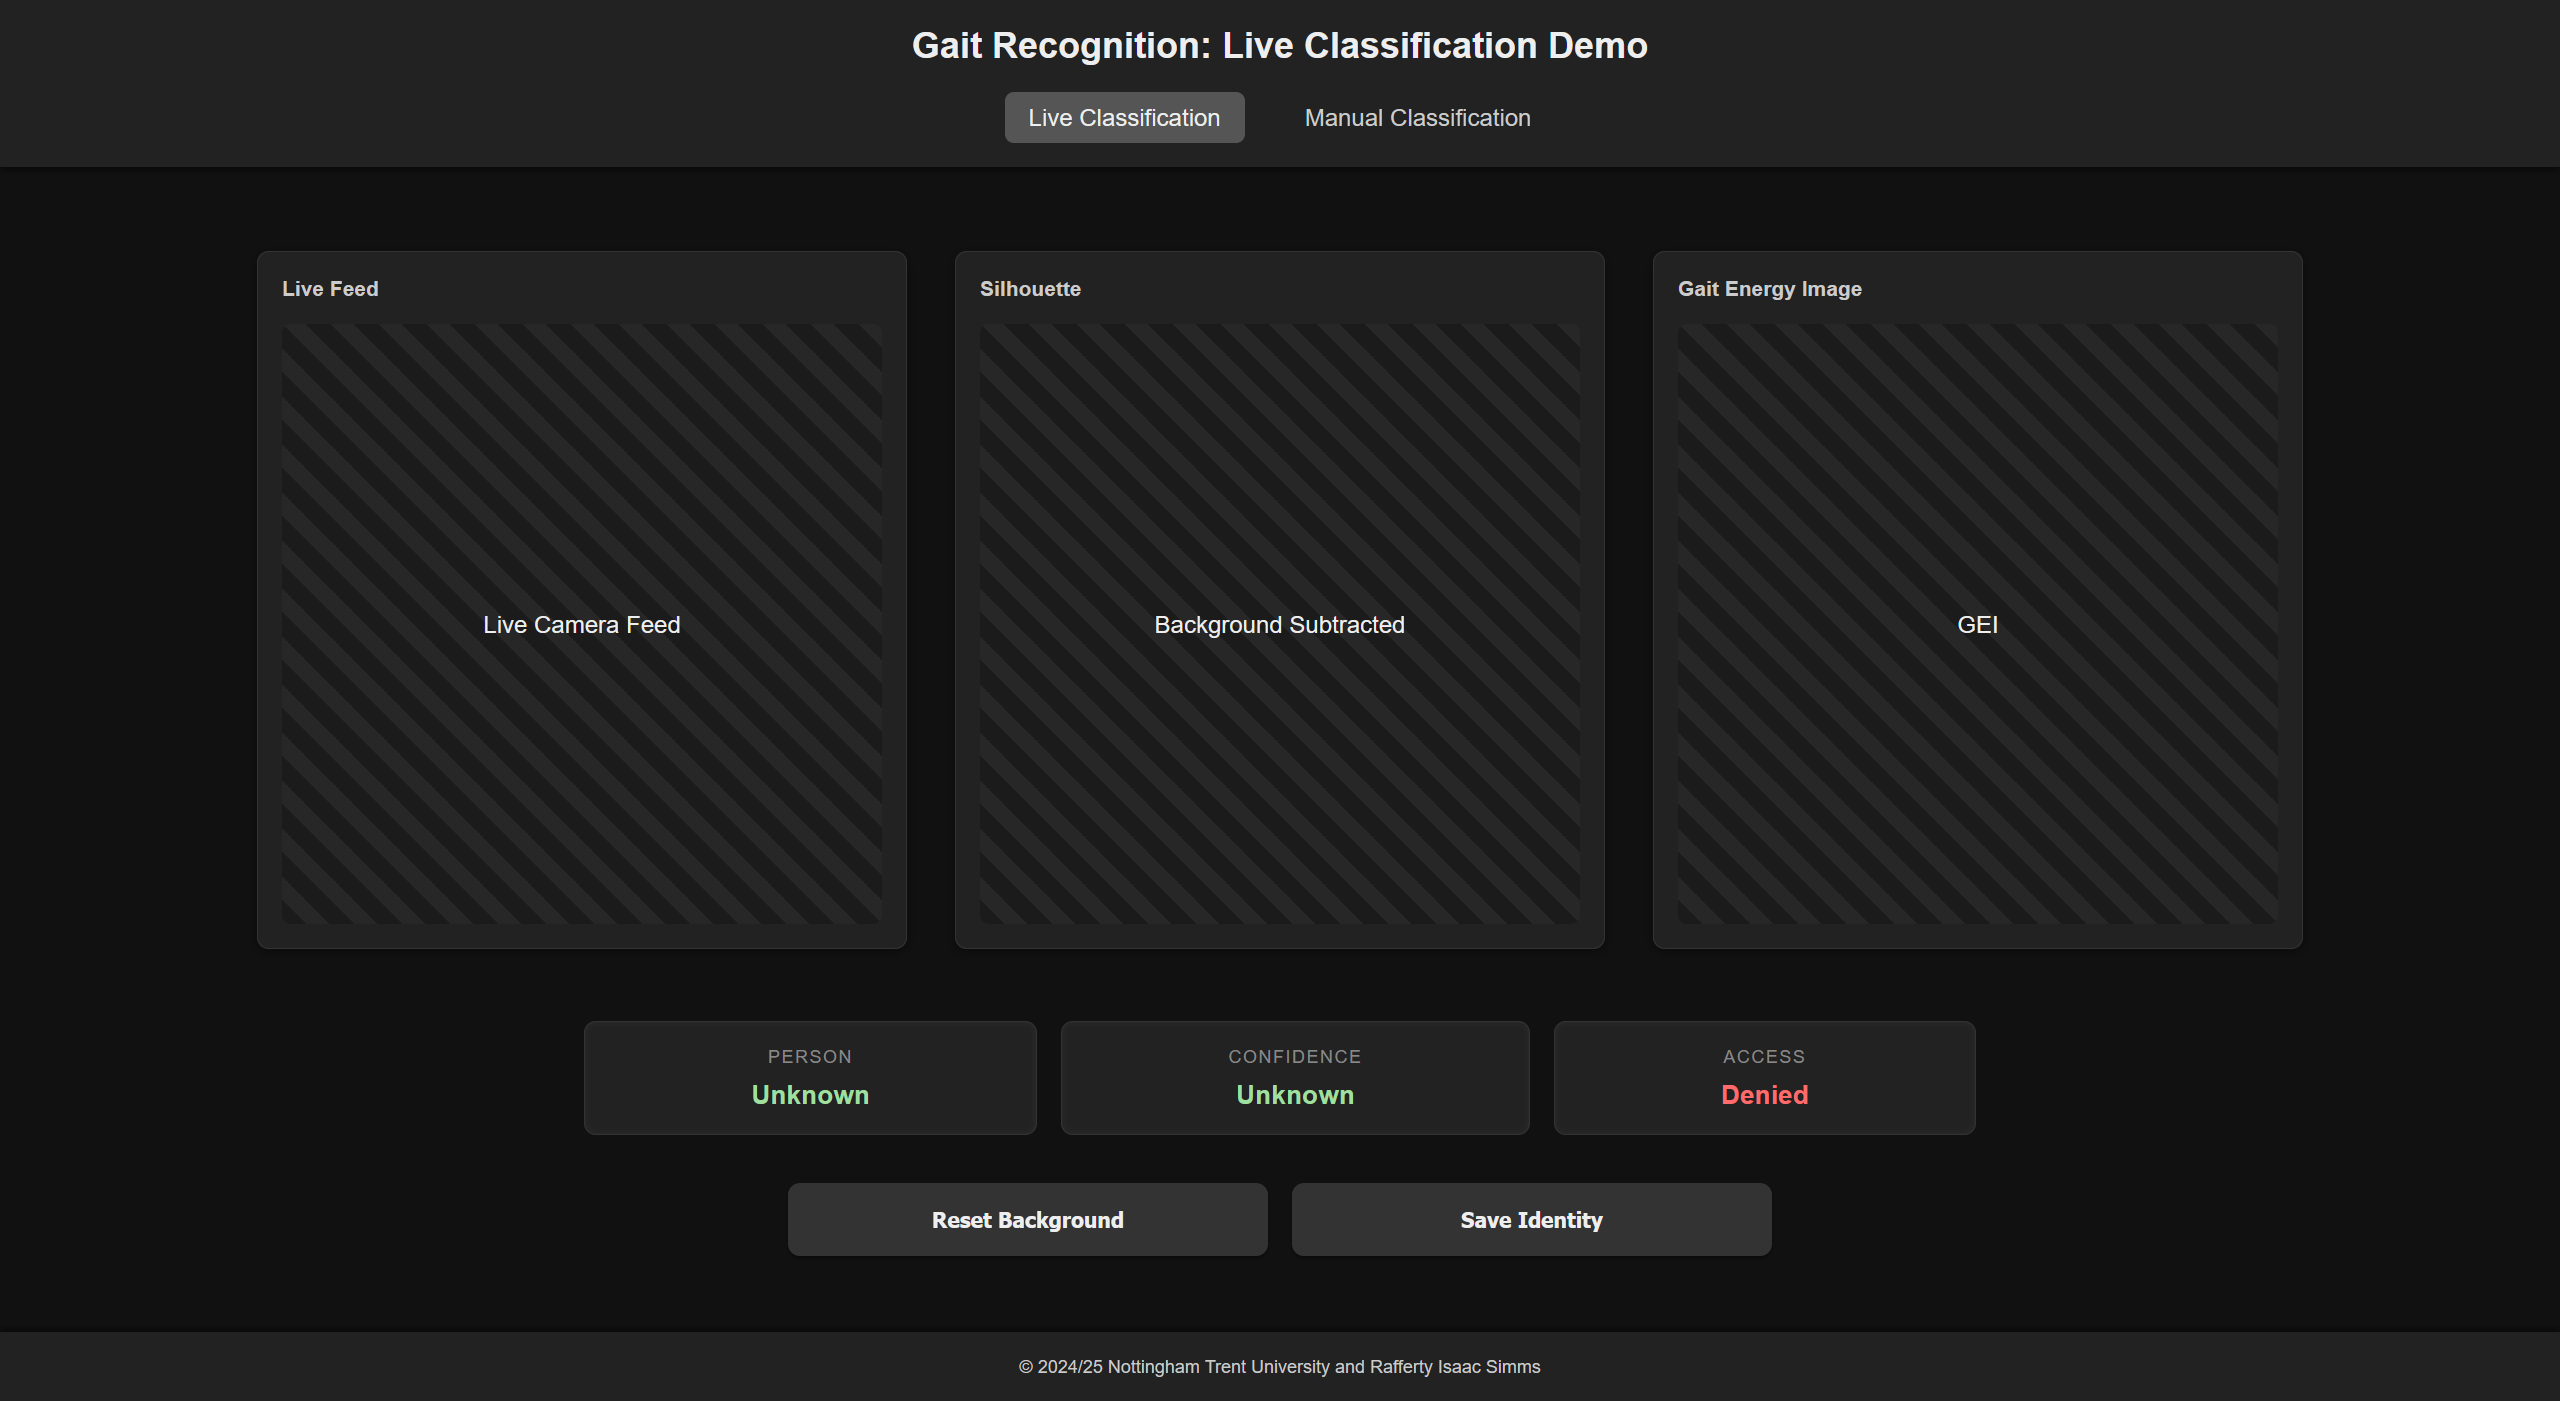
\includegraphics[width=0.9\textwidth]{assets/live-ui.png}
	\caption{Live Classification Page User-Interface}
	\label{fig:live-ui}
\end{figure}

The use of \ac{ws}s on this page allows for efficient data streaming from the back-end to update frame data or classification results without the overhead of additional HTTP headers.

The 'Manual Classification' page shown in the screenshot in Figure \ref{fig:manual-ui}, enables manual \ac{gei}-based identity classification, support for which was implemented in Section \ref{subsubsec:manual-classification-implementation}.
It features a 'drag-and-drop' area for image file submission, alongside a display of the uploaded image.
Below this, the same text views from the main page are used to present classification results returned by the \ac{grs}.

\begin{figure}[H]
	\centering
	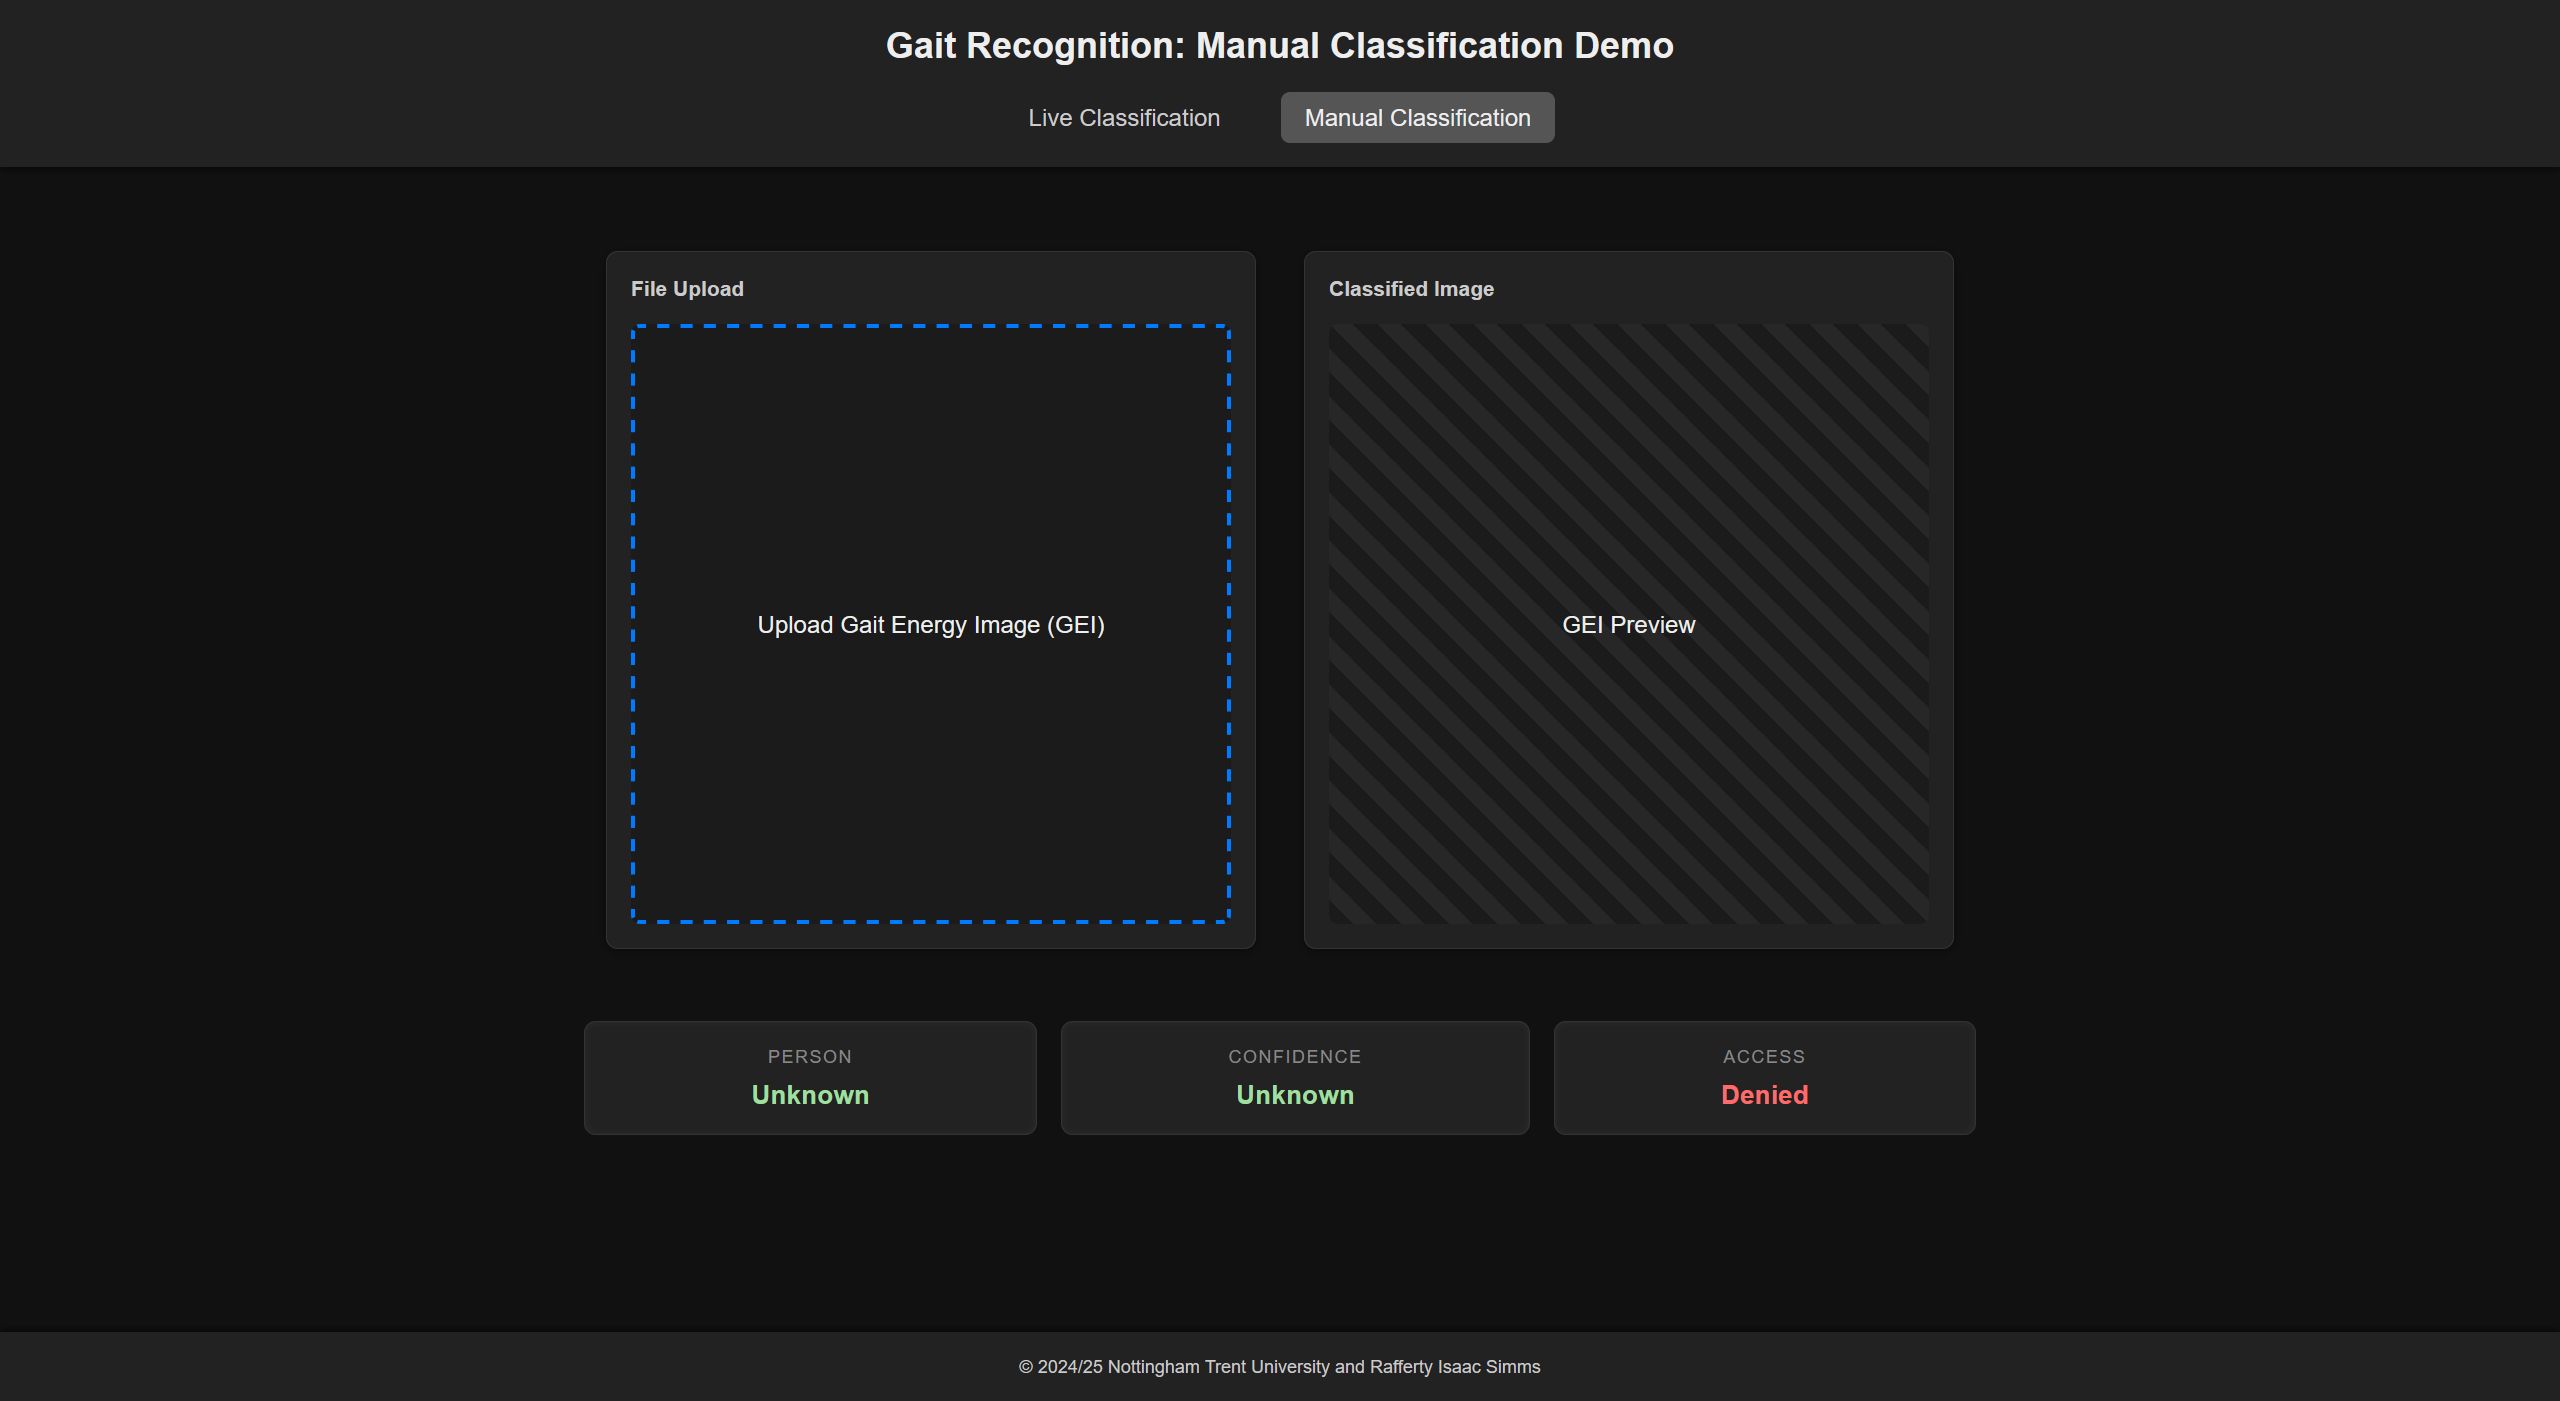
\includegraphics[width=0.9\textwidth]{assets/manual-ui.png}
	\caption{Manual Classification Page User-Interface}
	\label{fig:manual-ui}
\end{figure}

Implementation of the front-end \ac{ui} concluded development of the \ac{acc}.
It also fulfills the \ac{acc} ACF6 and ACF8 requirements, providing a \ac{ui} displaying the camera and \ac{gei} processing feeds, and displaying access decisions.
An evaluation of this component's adherence to the design and requirements is detailed in Section \ref{chap:results-and-evaluation}.


\subsection{Gait Recognition Server}
\label{subsec:gait-recognition-server-implementation}

\subsubsection{Database Modelling}
\label{subsubsec:database-modelling}

Following the database structure defined in Section \ref{subsubsec:database-design}, an SQLite database model has been implemented using the SQL Alchemy Python package.
A custom Python module named 'models' has been created, within which the below five classes are defined, inheriting from the SQL Alchemy \codeword{Model} class.
The database models module can be seen in full in Appendix \ref{app:database-models-implementation}.

The \codeword{Identity} class models individual identities registered in the system.
Each identity entry contains a unique \codeword{id}, a label, and establishes relationships with both the gait sample and access control rule tables. Referential deletes have been defined with these relationships, maintaining integrity when records are removed.

The \codeword{GaitSample} model stores individual \ac{gei} samples, each linked to an identity.
Each sample includes a \ac{gei} in Base64-encoded text format, a binary representation of its extracted features (see Section \ref{subsubsec:appearance-based-approaches}), and a timestamp marking its creation.
Implementation and this and the \codeword{Identity} table meets the \ac{grs} GRF4 requirement, maintaining historic movement data for each registered identity.

The \codeword{AccessRule} model associates Boolean access permissions (\codeword{True} for allow, \codeword{False} for deny) with a given identity. It enforces a one-to-one relationship with the \codeword{Identity} model by setting \codeword{identity\_id} as its primary key. This meets the \ac{grs} GRF5 requirement, allowing the system to manage access control rules for each registered identity.

The \codeword{GaitModel} class stores serialised data representing the trained \ac{pca} model used for \ac{gei} feature dimensionality reduction. It includes the binary-encoded \ac{pca} components, the mean vector, the current number of components, and the timestamps denoting model creation time and last update. In this implementation, only one model is stored in this table, with the values contributing to \ac{gei} classification.

The \codeword{ActivityLog} class is used for recording system activity, when identification occurs, or identities or gait samples are created or deleted, records are added to this table.
A page on the \ac{grs}' front-end then displays the logs for the user. Each log entry denotes the type of activity (e.g., 'identify'), optional descriptive details, and a timestamp.

Implementing the database model in a module allows it to be accessed and used in many areas throughout the \ac{grs} application by importing the database instance: \codeword{from models import db}. 
The following sections will refer to the use of this model when inserting, updating, or deleting database records.

\subsubsection{Feature Extraction, Model Training, and Classification}
\label{subsubsec:feature-extraction-model-training-and-classification}

Like the \ac{acc}'s gait processing features, gait-related functions in the \ac{grs} have been encapsulated into a single 'gait' module.
This module enables \ac{gei} feature extraction using a \ac{cnn}, \ac{pca} dimensionality reduction and model training, and \ac{gei}-based identity classification; processes discussed in more detail below.

\begin{tcolorbox}[colback=red!5, boxrule=0pt, frame empty]
	\paragraph{Issue Encountered!} A model-free $k$-\ac{nn} approach was originally implemented at this stage. The idea being that for a \ac{poc}, the classification did not have to be perfect, and a model-free matching algorithm could be used for demonstration purposes.
	Unfortunately, testing showed this was highly susceptible to overfitting, meaning the chance of misclassification, especially with smaller datasets was higher than acceptable.
	Because of this, the decision was made to commit to implementing an \ac{ml} model-based classification scheme, with a \ac{cnn}, \ac{pca}, and cosine similarity pipeline implemented in the final solution.
\end{tcolorbox}

Feature extraction is achieved using a \ac{cnn} with the pretrained \codeword{EfficientNetB0} model through the 'TensorFlow' Python package (see Listing \ref{lst:feature-extraction}) after being transformed to expected resolution and colour format (224x224 and RGB) using \ac{cv2}.
This model provides a good trade-off between performance and efficiency compared to more demanding options like \codeword{VGG16} --- ideal for this demonstrative scenario.

\begin{code}
base_model = EfficientNetB0(weights="imagenet", include_top=False)
feature_extractor = Model(inputs=base_model.input, outputs=base_model.get_layer("top_conv").output)
...
batch = np.expand_dims(gei, axis=0)
features = feature_extractor.predict(batch, verbose=0)
\end{code}
\captionof{listing}{Feature Extraction Model Definition and Usage}
\label{lst:feature-extraction} \vspace{10pt}

After processing, the \ac{cnn} output is flattened forming a 'feature vector' representing the input \ac{gei}: \codeword{features.flatten()}.
These features are stored in the database alongside other sample information in the \codeword{GaitSample} table when a new \ac{gei} is registered (see Section \ref{subsubsec:database-design}).

To improve classification speed and accuracy, \ac{pca} is applied to reduce the dimensionality of \ac{cnn}-extracted features (see Section \ref{subsubsec:classification-techniques}).
A 'trained' \ac{pca} model is stored in the database and updated every time a new \ac{gei} sample is added using the \codeword{update\_model} function.
This retrieves all samples from the database before standardising features using the 'scikit-learn' Python module's \codeword{StandardScaler} --- ensuring equal structure and fair \ac{pca} evaluation.
The number of \ac{pca} components is chosen dynamically based on the size of the dataset: $\min(128, \mathit{dataset\_size}-1)$.
Listing \ref{lst:pca-model-training} below demonstrates the creation of a scaled list of all features, and training of a \ac{pca} model based on the standardised features. 

\begin{code}
features = np.array([pickle.loads(sample.features) for sample in gait_samples])

scaler = StandardScaler()
features_scaled = scaler.fit_transform(features)

n_components = min(128, len(features) - 1)
pca = PCA(n_components=n_components)
pca.fit(features_scaled)
\end{code}
\captionof{listing}{PCA Model Training Logic}
\label{lst:pca-model-training} \vspace{10pt}

Dimension-reduced \ac{pca} components and its the 'mean vector' are then serialised using the Python 'pickle' module and stored in \codeword{pca\_components} and \codeword{mean\_vector} fields of the database's \codeword{GaitModel} table, improving future classification performance by reducing redundant computation of each sample when performing comparisons.

The third function provided by this module --- \codeword{classify} --- enables classification of \ac{gei}s.
It accepts a single \ac{gei} as input before calling the \codeword{extract\_features} function to retrieve its \ac{cnn} features.
Following this, the \ac{pca} model is retrieved from the \codeword{GaitModel} table and decoded from binary.
The features of the input \ac{gei} are then scaled and projected according to the \ac{pca} model's components and mean vector, as shown in Listing \ref{lst:feature-extraction-and-pca-projection}. 

\begin{code}
features = extract_features(gei)
gait_model = GaitModel.query.first()

pca_components = pickle.loads(gait_model.pca_components)
mean_vector = pickle.loads(gait_model.mean_vector)

features_scaled = (features - mean_vector) / np.sqrt(np.var(features))
projected_features = np.dot(features_scaled, pca_components.T)
\end{code}
\captionof{listing}{Feature Extraction and PCA Projection Logic}
\label{lst:feature-extraction-and-pca-projection}
\vspace{10pt}

After the input \acp{gei} features have been extracted and the \ac{pca} model loaded, all existing samples are loaded and iterated through with the 'cosine similarity' (calculated by calculating the cosine of the angle between the feature vector of the input and each sample) to the input calculated for each, using the scikit-learn module's \codeword{cosine\_similarity} function once they have been scaled and projected to fit the \ac{pca} model structure.
This process is illustrated below in Listing \ref{lst:cosine-gei-similarity-comparison}. 

\begin{code}
for sample in gait_samples:
	sample_features = pickle.loads(sample.features)
	sample_features_scaled = (sample_features - mean_vector) / np.sqrt(
		np.var(sample_features)
	)
	sample_projected = np.dot(sample_features_scaled, pca_components.T)

	similarities.append(
		(
			cosine_similarity(
				projected_features.reshape(1, -1),
				sample_projected.reshape(1, -1),
			)[0][0],
			sample.identity.label if sample.identity else None,
		)
	)
\end{code}
\captionof{listing}{Cosine Similarity Comparison between Input and Samples}
\label{lst:cosine-gei-similarity-comparison} \vspace{10pt}

Finally, the best match is selected from the list of similarities, and the confidence is calculated as a percentage of the best match's similarity.
The function then returns the predicted label and confidence.
This meets the \ac{grs} GRF2 and GRF10 requirements, allowing the system to classify (predict the identity of) \ac{gei} samples using a trained \ac{ml} model.

\subsubsection{Identity Registration Endpoint}
\label{subsec:identity-registration-endpoint}

\ac{gei}-based identity registration functionality is provided to the \ac{acc} via the \ac{grs}' \ac{api} endpoint at \codeword{/api/register}, implemented using the Flask web framework.
This endpoint accepts \codeword{POST} requests containing a \ac{json} object with two fields: a Base-64-encoded \ac{gei} and the identity label entered by the user on the client side.

Upon receiving a request, the handler function first checks whether an identity with the specified label already exists in the database.
If not, a new \codeword{Identity} entry is created and saved, with a default \codeword{AccessRule} entry also initialised for the new identity, set to \codeword{False} (i.e., access denied by default).

The \ac{gei} is then decoded from its Base64 representation and passed to the \codeword{extract\_features} function (see Section \ref{subsubsec:feature-extraction-model-training-and-classification}), which extracts a feature vector using the EfficientNetB0 \ac{cnn}.
The extracted features are serialised using the 'pickle' module, and a new \codeword{GaitSample} record is created and populated accordingly.
At the same time, a new \codeword{ActivityLog} entry is created of type 'register' to log the registration event.
This is shown in Listing \ref{lst:identity-registration} below. 

\begin{code}
gei = base64.b64decode(base64_gei)
nparr = np.frombuffer(gei, np.uint8)
gei = cv2.imdecode(nparr, cv2.IMREAD_GRAYSCALE)

features = extract_features(gei)
serialized_features = pickle.dumps(features)

new_sample = GaitSample(identity_id=identity.id, gei_image=base64_gei, features=serialized_features, created_at=datetime.now())
db.session.add(new_sample)

activity_log = ActivityLog(activity_type="register", details=str({"label": label}), created_at=datetime.now())
db.session.add(activity_log)
\end{code}
\captionof{listing}{Identity Registration Endpoint Logic}
\label{lst:identity-registration} \vspace{10pt}

Finally, the \codeword{update\_model} function is called to retrain the \ac{pca} model using the updated dataset (see Section \ref{subsubsec:feature-extraction-model-training-and-classification}), before a \ac{json} response is returned to the client containing the ID of the affected identity.
This meets the \ac{grs} GRF1 requirement, supporting the registration of new identities and \ac{gei} samples.

\subsubsection{Identity Classification Endpoint}
\label{subsec:identity-classification-endpoint}

The \ac{grs} handles \ac{gei} classification requests from the \ac{acc} via the \codeword{/api/classify} \ac{api} endpoint.
The endpoint accepts \codeword{POST} requests containing a \ac{json} object with a single Base64-encoded \ac{gei}.

Upon receiving a request, the handler function decodes the \ac{gei} from Base64 and passes it to the \codeword{classify} function (see Section \ref{subsubsec:feature-extraction-model-training-and-classification}) to retrieve the predicted identity label and confidence score reflecting prediction certainty: \codeword{prediction, confidence = classify(gei)}.

Following identity prediction, the system retrieves the corresponding access rule for the predicted identity from the AccessRule table.
An \codeword{ActivityLog} entry of type 'identify' is created to record the classification event, including both the predicted identity and the associated confidence score.

Finally, the \ac{grs} responds to the client with a \ac{json} object containing three fields: the predicted identity, the confidence score, and the access rule.
A successful response is shown in Listing \ref{lst:identity-classification-response} below.
This meets the \ac{grs} GRF3 and GRF9 requirements, responding to \ac{acc} queries with the predicted identity, and logging the event. 

\begin{code}[minted language=text]
"success": True,
"person": prediction,
"confidence": float(confidence),
"access": access_granted,
\end{code}
\captionof{listing}{Identity Classification Endpoint (Successful) Response}
\label{lst:identity-classification-response} \vspace{10pt}


\subsubsection{Access Control Rule Management}
\label{subsubsec:access-control-rule-management}

Access rule configuration is enabled via toggle switches in the front-end \ac{ui} (see Section \ref{subsec:access-control-client-design}), and implemented using Socket.IO-based \acf{ws}.

On the back-end, access rule updates are handled by the \codeword{handle\_access\_rule\_update} Socket.IO listener.
This expects transmissions to contain two fields: an \codeword{identity\_id} integer and an \codeword{allow\_access} Boolean.
The \ac{grs} uses the provided \codeword{identity\_id} to query the corresponding identity from the database and updates the associated \codeword{AccessRule} entry's \codeword{rule} field to reflect the new status.
This is shown in Listing \ref{lst:access-rule-update-logic} below.

\begin{code}
identity = Identity.query.get_or_404(identity_id)
identity.access_rule.rule = allow_access
\end{code}
\captionof{listing}{Access Rule Update Logic}
\label{lst:access-rule-update-logic} \vspace{10pt}

On the front-end, each identity's page includes a toggle switch linked to a \ac{js} function (shown in Listing \ref{lst:access-rule-toggle-frontend}) that is triggered whenever the toggle is clicked.
This function emits a \ac{ws} message containing the toggle's Boolean state and the relevant identity's ID to the back-end.

\begin{code}[minted language=javascript]
const accessToggle = document.getElementById('accessToggle');

accessToggle.addEventListener('change', function (e) {
	const identityId = this.dataset.identityId;
	const allowAccess = this.checked;

	socket.emit('update-access-rule', {
		identity_id: identityId,
		allow_access: allowAccess
	});
});
\end{code}
\captionof{listing}{Access Rule Toggle Front-End Handler}
\label{lst:access-rule-toggle-frontend} \vspace{10pt}

The \ac{grs} front-end is designed to function independently of the \ac{acc}, allowing configuration changes to be made regardless of whether the \ac{acc} is running, meeting the \ac{grs} GRF7 requirement.

\subsubsection{Identity and Gait Cycle Management}
\label{subsec:identity-and-gait-cycle-management}

The \ac{grs}' \ac{ui} provides functionality for deleting either entire identities or individual gait cycles associated with an identity.
This functionality is also enabled through \ac{ws}-based communication and supported on the back-end via two Socket.IO event handlers: \codeword{handle\_delete\_identity} and \codeword{handle\_delete\_gait\_sample}.

The \codeword{handle\_delete\_identity} function expects a transmission containing an \codeword{identity\_id} integer.
This is used to retrieve the corresponding \codeword{Identity} entry from the database.
An \codeword{ActivityLog} entry of type 'delete' is then created to record the deletion event, including the label of the identity.
The identity is then removed from the database, and due to the configured database model relationships (see Section \ref{subsubsec:database-design}), the associated \codeword{AccessRule} and \codeword{GaitSample} records are also removed.
This is shown in Listing \ref{lst:identity-deletion-logic} below. 

\begin{code}
identity = Identity.query.get_or_404(identity_id)

activity_log = ActivityLog(
	activity_type="delete",
	details=str({"label": identity.label}),
	created_at=datetime.now(),
)
db.session.add(activity_log)

db.session.delete(identity)
\end{code}
\captionof{listing}{Identity Deletion Logic}
\label{lst:identity-deletion-logic} \vspace{10pt}

On the front-end, a delete button is placed in the top right corner of each identity's page.
When clicked, a \ac{js} function (shown in Listing \ref{lst:identity-deletion-frontend}) is triggered, prompting the user to confirm the deletion.
If confirmed, the \codeword{identity\_id} is emitted to the back-end over the \ac{ws} connection.

\begin{code}[minted language=javascript]
	const deleteIdentityBtn = document.getElementById('deleteIdentity');

	deleteIdentityBtn.addEventListener('click', function () {
		if (confirm('Are you sure you want to delete this identity?')) {
			const identityId = this.dataset.identityId;
			socket.emit('delete-identity', { identity_id: identityId });
		}
	});
\end{code}
\captionof{listing}{Identity Deletion Front-End Handler}
\label{lst:identity-deletion-frontend} \vspace{10pt}

For individual \ac{gei} deletion, the \codeword{handle\_delete\_gait\_sample} function is used. 
It accepts a \codeword{sample\_id} integer, retrieves the relevant \codeword{GaitSample} record from the database, and performs similar actions as with identity deletion: logging the deletion event via a new \codeword{ActivityLog} entry and removing the sample record from the \codeword{GaitSample} table: \codeword{db.session.delete(sample)}.

On the front-end, each \ac{gei} preview on the identity page includes a delete button.
Clicking this triggers a \ac{js} function similar to Listing \ref{lst:identity-deletion-frontend} that prompts the user for confirmation, then emits the corresponding \codeword{sample\_id} to the back-end via the \ac{ws} connection.

The final step for both handlers is to call the \codeword{update\_model} function (see Section \ref{subsubsec:feature-extraction-model-training-and-classification}) to retrain the \ac{pca} model on the updated dataset, ensuring no redundant data is included that may affect accuracy.


\subsubsection{Statistic and Log Processing}
\label{subsubsec:statistic-and-log-processing}

The \ac{grs} includes an independent 'Statistics \& Logs' page, providing an overview of system activity.
When the page is accessed, the back-end queries the total number of entries in the \codeword{Identity} and \codeword{GaitSample} tables and retrieves entries from the \codeword{ActivityLog} table in descending creation order.

Once retrieved, the logs are processed into a \codeword{formatted\_logs} list, where each entry is transformed into a human-readable message summarising the action performed (e.g., identity registration, classification, or deletion).

Finally, the stats page (see Section \ref{subsec:gait-recognition-server-user-interface}) is rendered with the identity count, \ac{gei} sample count, and the list of formatted log messages passed as parameters to the front-end, where they are displayed in an accessible format.

The logic for retrieving and formatting the statistic and log data can be seen in Appendix \ref{app:activity-log-retrieval-and-formatting}.

\subsubsection{User-Interface}
\label{subsec:gait-recognition-server-user-interface}

The \ac{grs}'s front-end --- comprising the three pages designed in Section \ref{subsubsec:server-ui-design} --- is built using the same technologies as the \ac{acc}'s front-end.
It enables users to manage registered identities and their associated \ac{gei} samples, configure access control rules, and view system statistics and logs.

The 'Server Home' (index) page, shown in the screenshot in Figure \ref{fig:server-home}, presents a grid view of all registered identities.
Selecting an identity navigates the user to the 'Identity' page outlined below.
Each identity card includes the identity's label, the most recent \ac{gei} sample added, the creation date, and a Boolean flag indicating access status.

\begin{figure}[H]
	\centering
	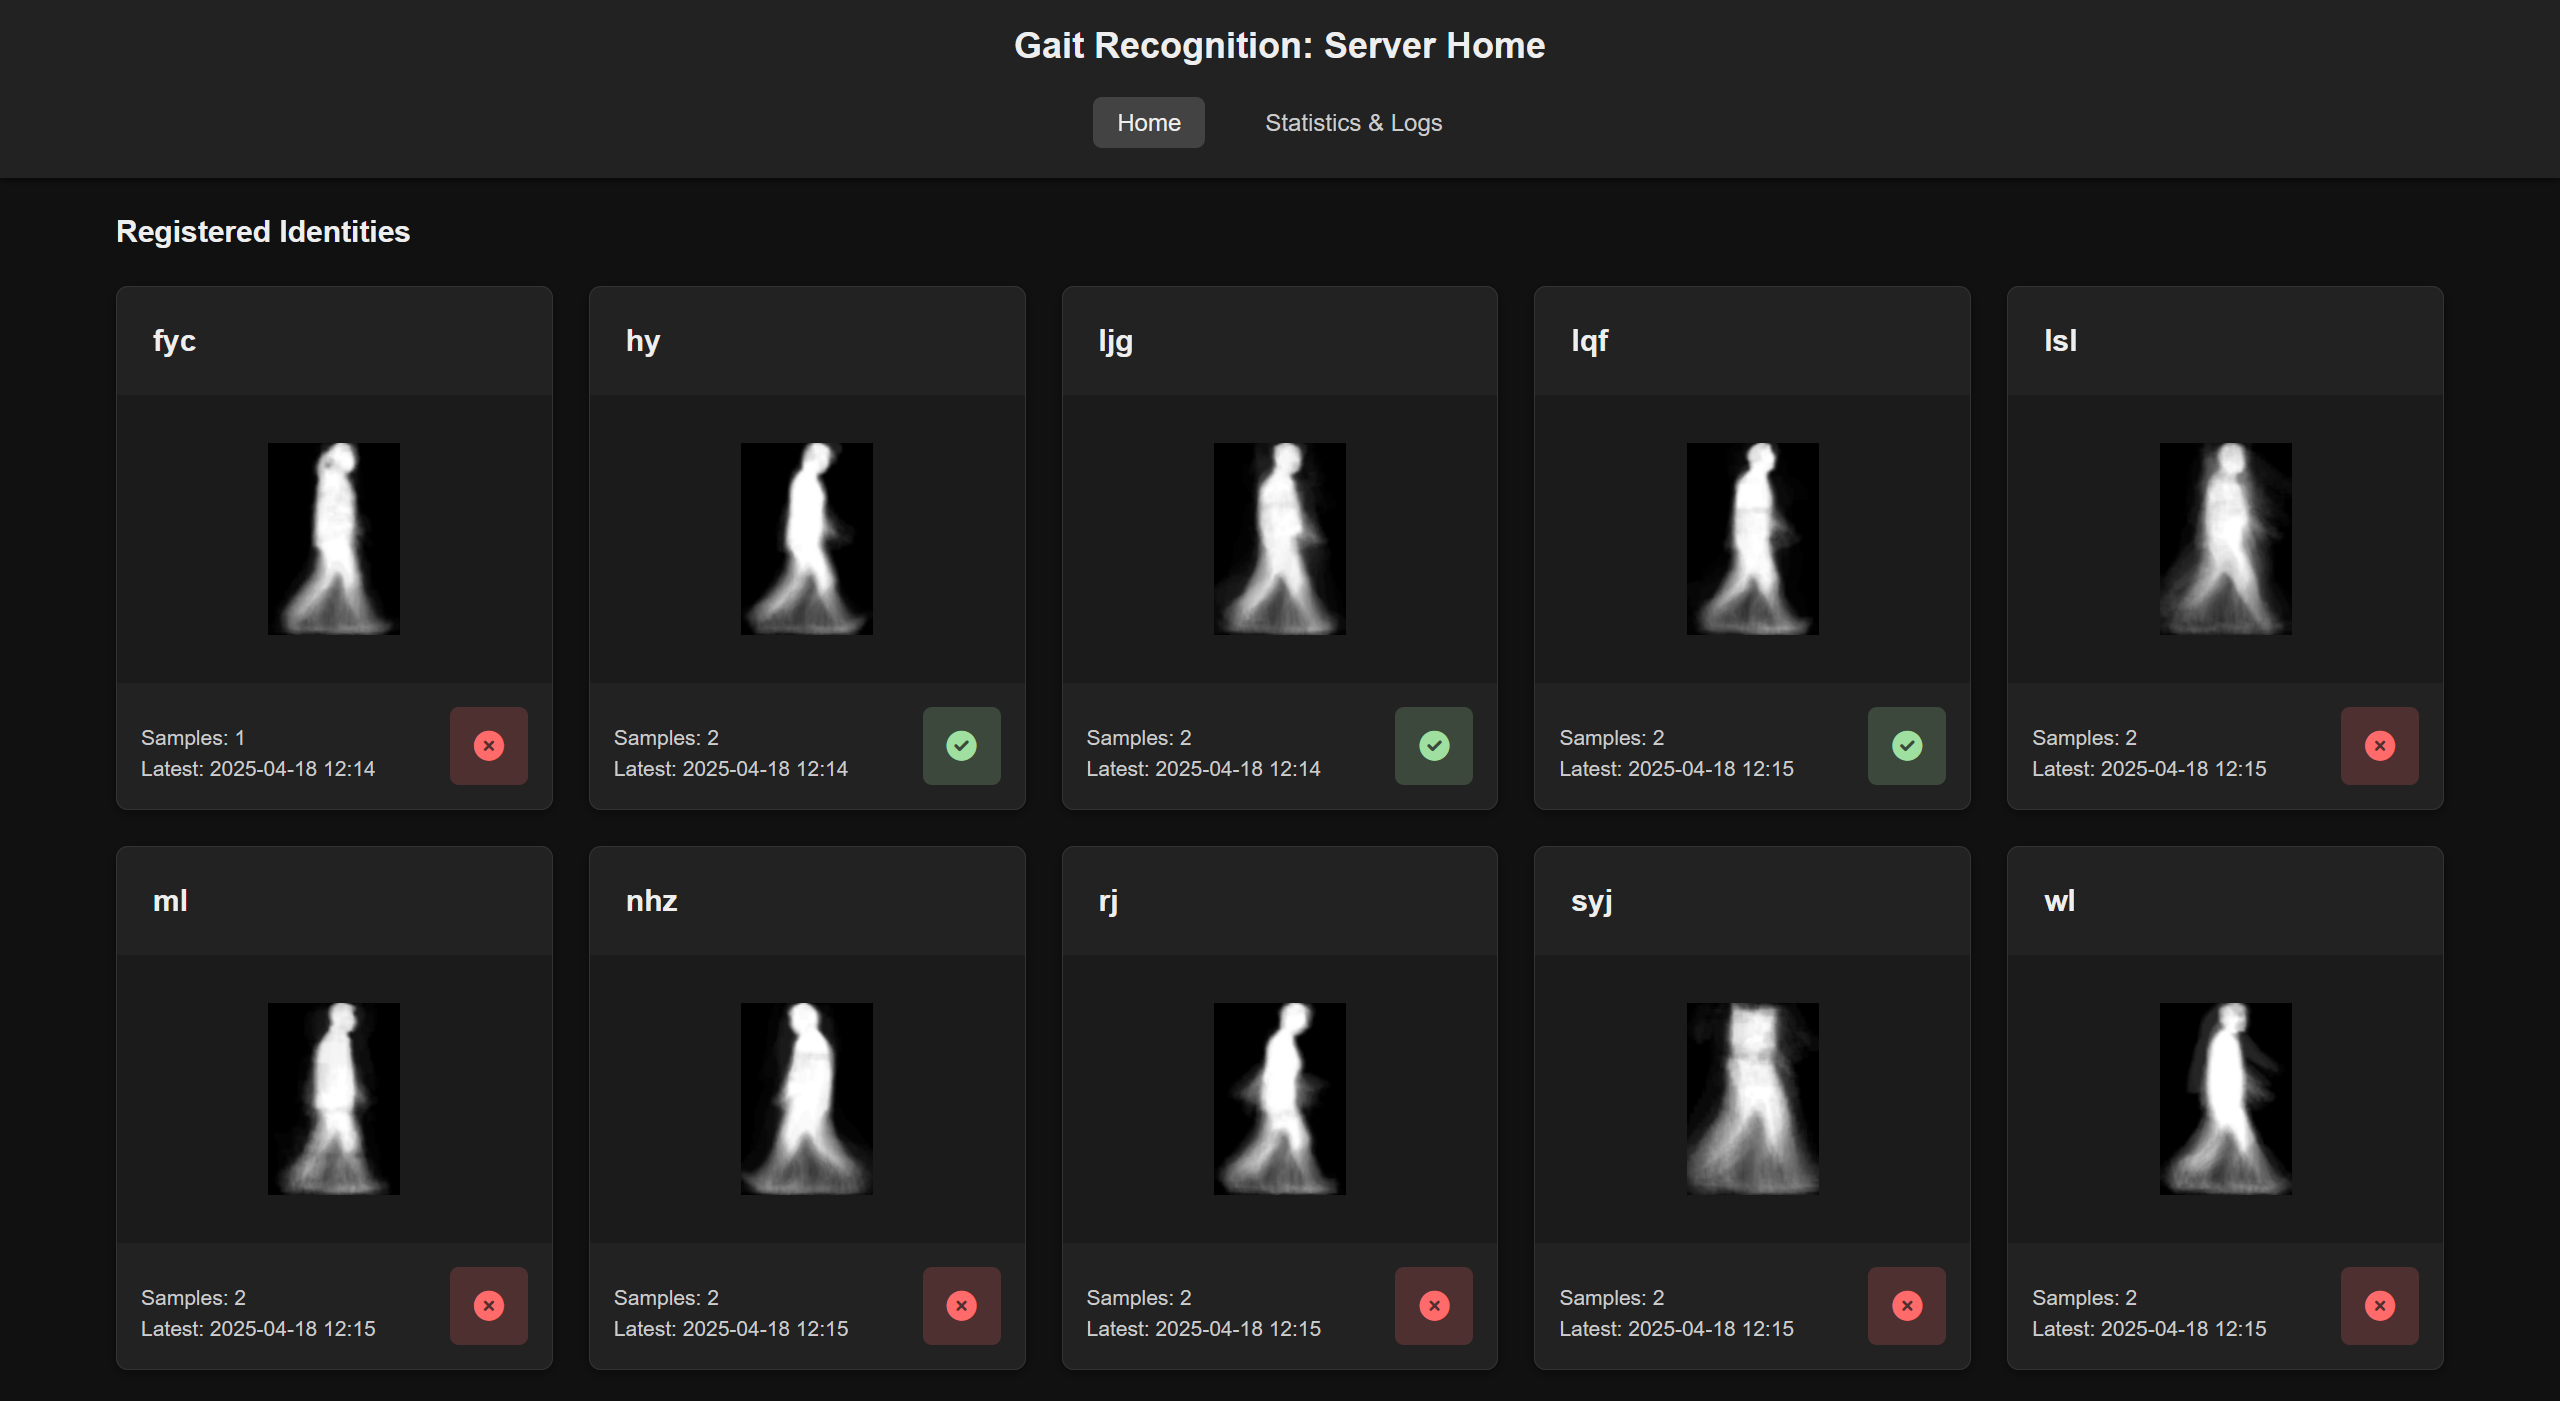
\includegraphics[width=0.9\textwidth]{assets/server-home.png}
	\caption{'Server Home' Page User-Interface}
	\label{fig:server-home}
\end{figure}

The 'Identity' page, shown in Figure \ref{fig:identity-page}, displays detailed information about the selected identity, including the identity ID, number of \ac{gei} samples, creation date, and last update timestamp.
A toggle switch allows configuration of the access rule for the identity, and a delete button enables removal of the identity (see Section \ref{subsec:identity-and-gait-cycle-management} for deletion logic).
Below this, a grid displays all \ac{gei} samples associated with the identity, with individual delete buttons allowing selective removal of specific samples.

\begin{figure}[H]
	\centering
	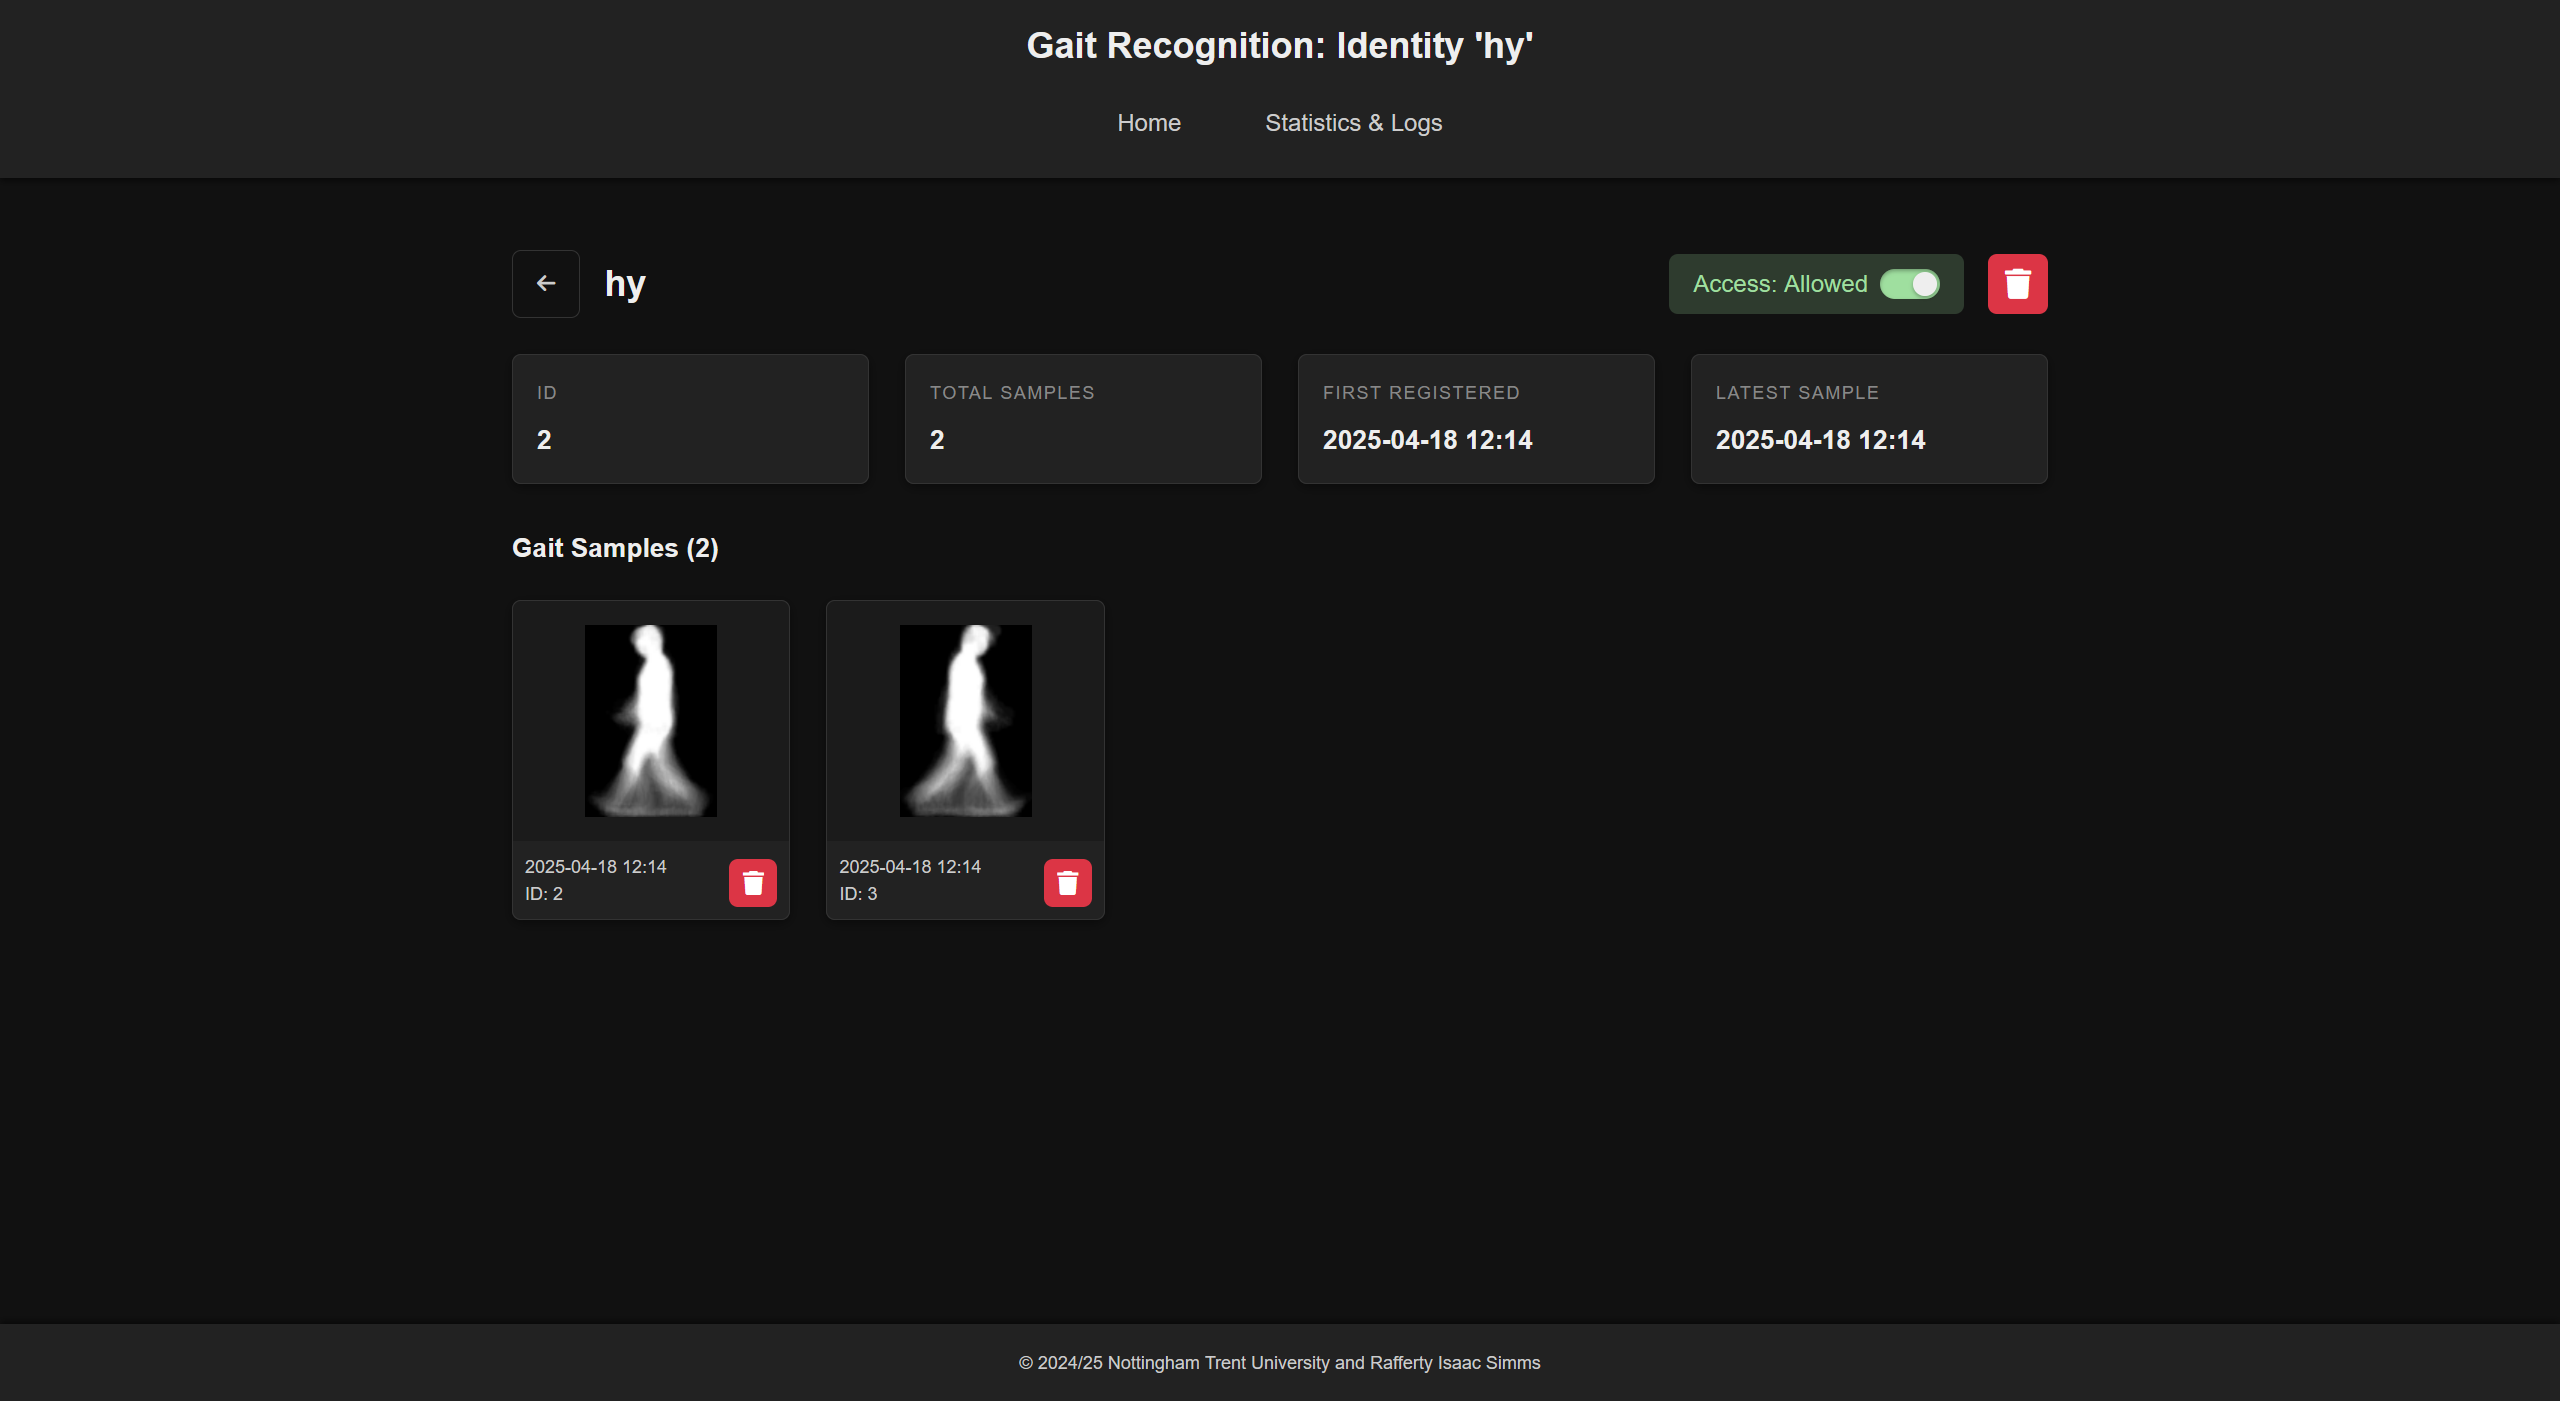
\includegraphics[width=0.9\textwidth]{assets/identity-page.png}
	\caption{'Identity' Page User-Interface}
	\label{fig:identity-page}
\end{figure}

The 'Statistics \& Logs' (stats) page, shown in Figure \ref{fig:stats-page}, presents a summarised view of the system's state.
A row of three metrics --- the total number of registered identities, total number of \ac{gei} samples, and average number of \ac{gei} samples per identity --- is displayed at the top.
Below that, a chronological list of activity logs is provided, in descending creation order.

\begin{figure}[H]
	\centering
	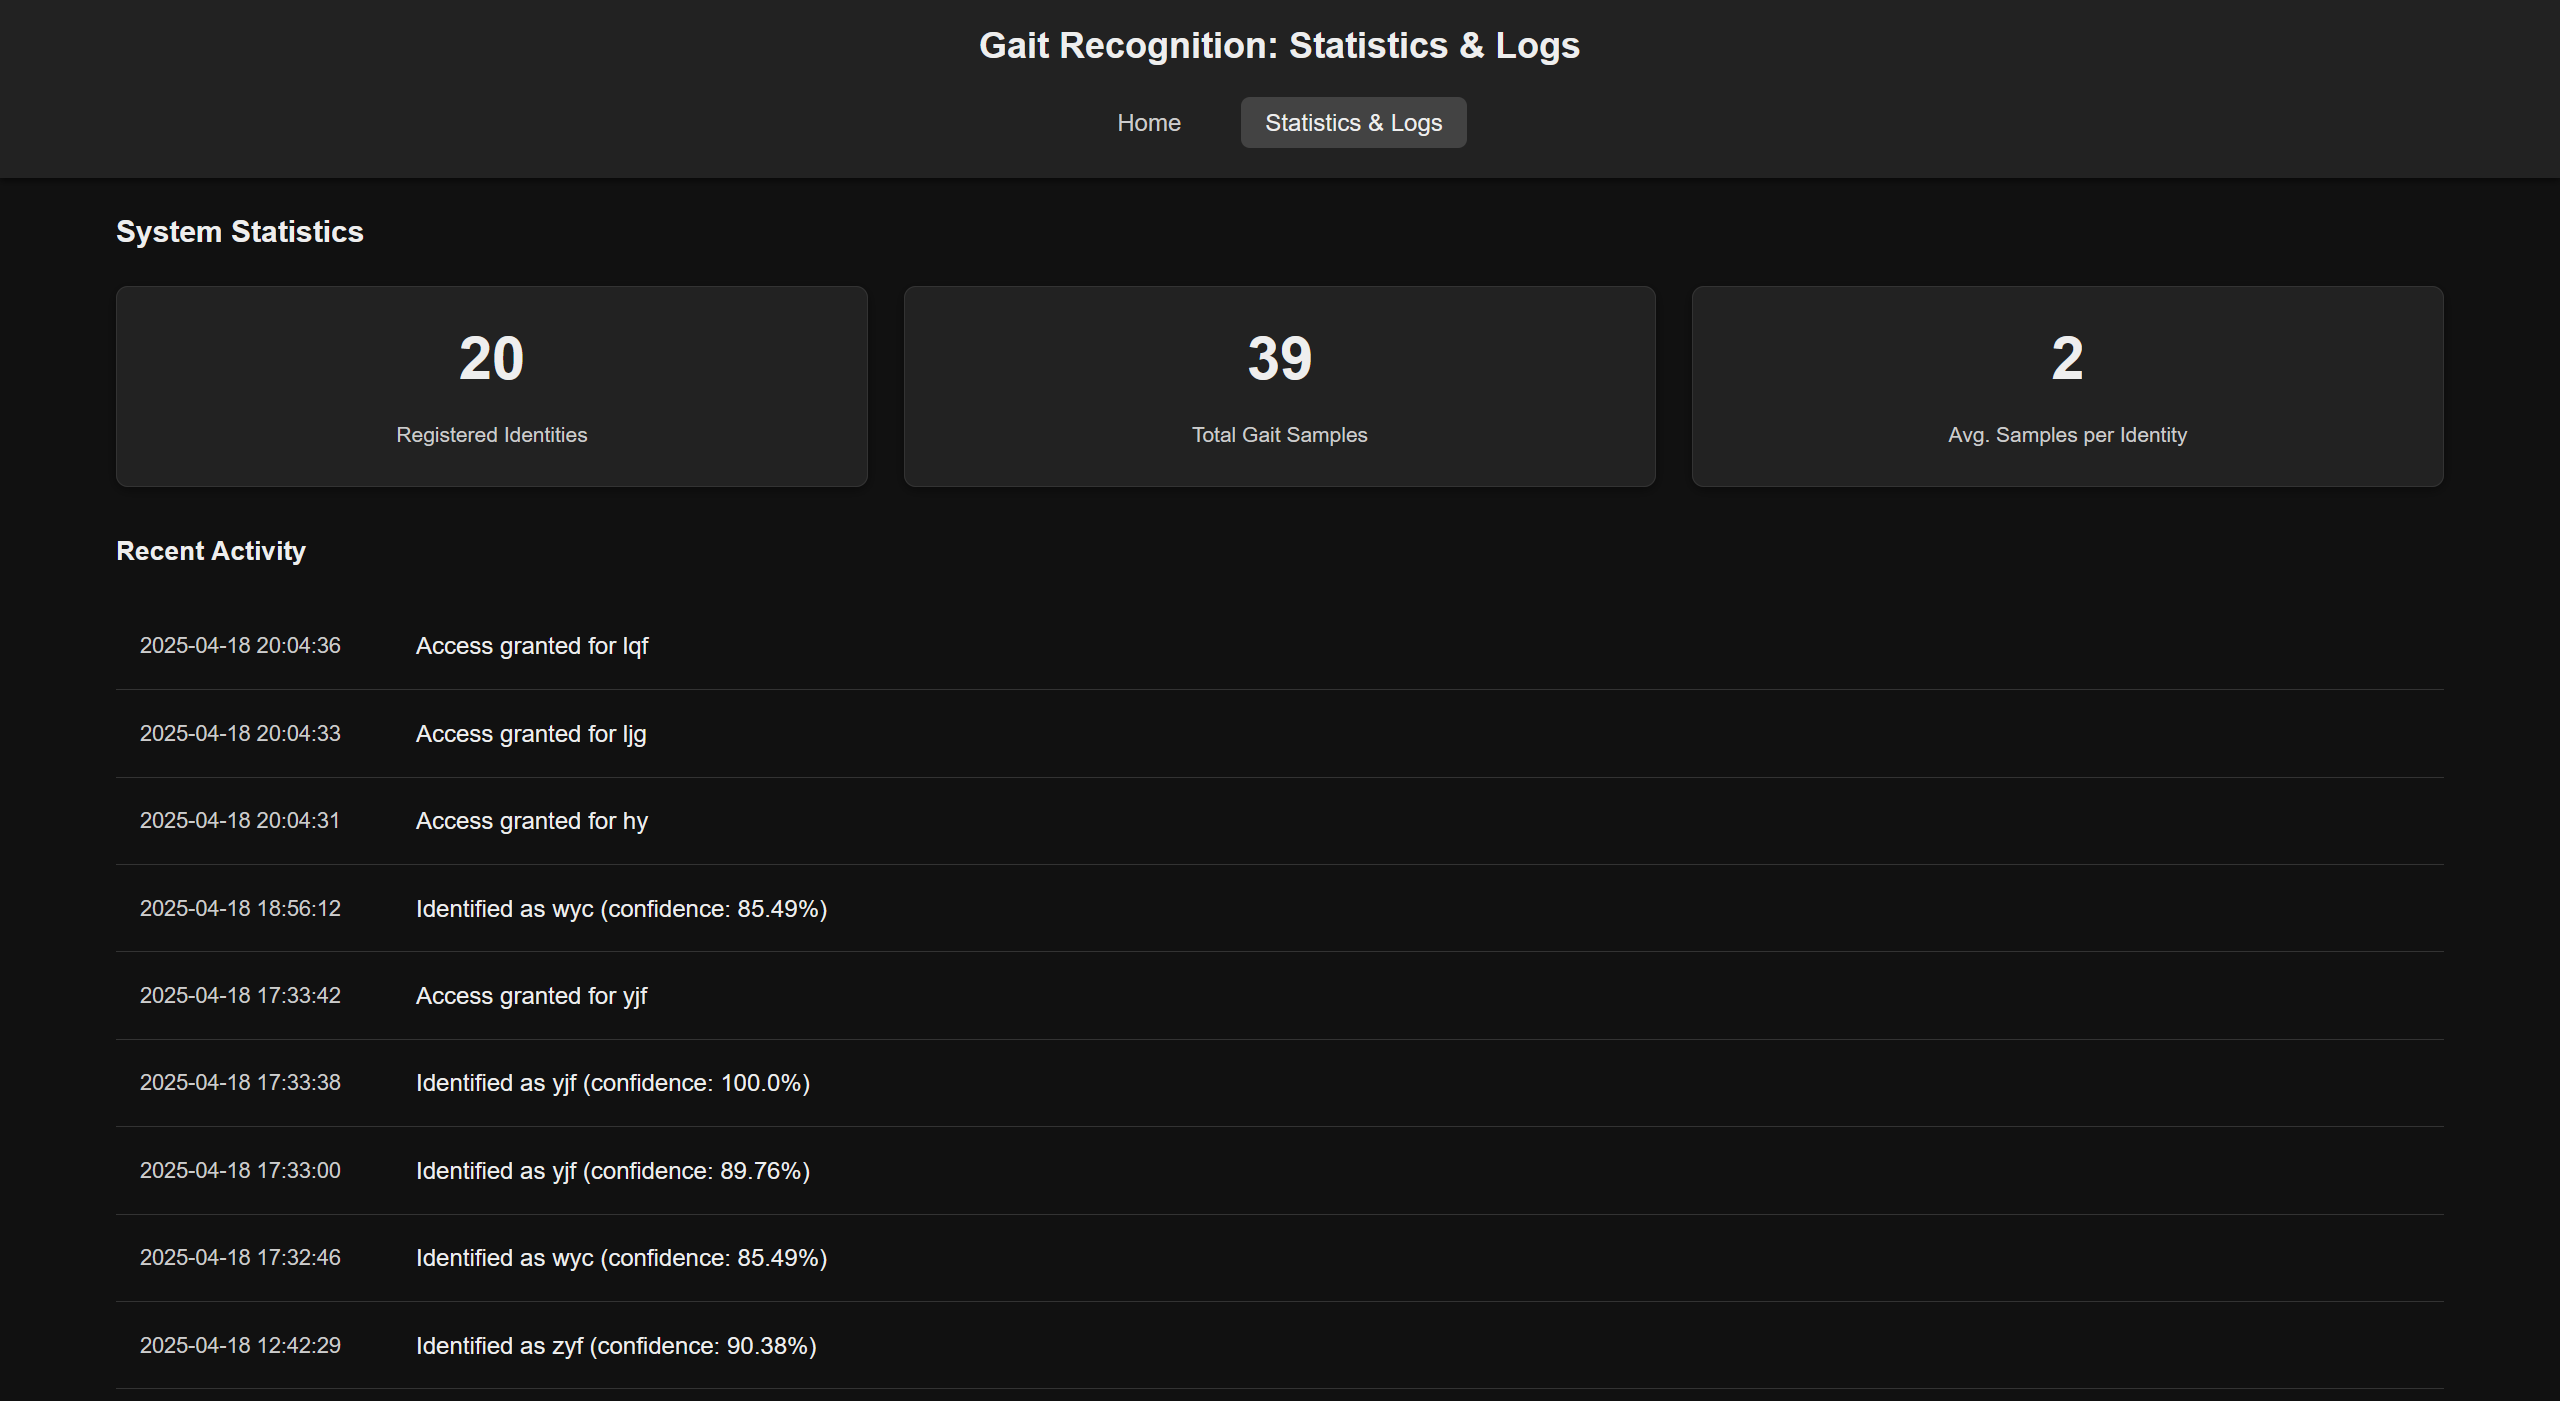
\includegraphics[width=0.9\textwidth]{assets/stats-page.png}
	\caption{'Statistics \& Logs' Page User-Interface}
	\label{fig:stats-page}
\end{figure}

Implementation of the server-side \ac{ui} concluded development of the gait recognition server and overall project.
Adherence of this component to the functional requirements defined in Chapter \ref{chap:new-ideas}, along with evaluation results regarding classification performance and accuracy, are discussed in Section \ref{chap:results-and-evaluation}.

Overall, only one major issue was encountered during implementation: the original choice of a model-free $k$-\ac{nn} approach for \ac{gei} classification was highly susceptible to overfitting (discussed in Section \ref{subsubsec:feature-extraction-model-training-and-classification}), meaning the chance of misclassification, especially with smaller datasets was higher than acceptable. However, this issue was quickly resolved thanks to the software development methodology being used, allowing revisions to be made quickly.